\documentclass[a4paper]{article}
\usepackage[english]{babel}
\usepackage{ucs}
\usepackage[utf8x]{inputenc}
\usepackage[T1]{fontenc}
\usepackage{times}
\usepackage[pdftex]{graphicx}
\usepackage{color}
\usepackage[pdftex,colorlinks=true,citecolor=black,
            pagecolor=black,linkcolor=black,menucolor=black,
            urlcolor=black]{hyperref}
%\usepackage{eufrak}
\usepackage{amsmath}
\usepackage{amsbsy}
\usepackage{eucal}
\usepackage{subfigure}
\usepackage{longtable}
\usepackage{url}
\urlstyle{same}
\usepackage{verbatim} % For verbatiminput.

\usepackage{amssymb}

\usepackage{natbib}
\usepackage{chngpage}

\pdfinfo{            
          /Title      (Project assignment for T-61.3015 Digital 
          Signal Processing)
          /Author     ()
          /Keywords   ()          
}

\begin{document}

\title{Project assignment \\
T-61.3015 Digital Signal Processing}
\author{Jarno Alanko \\
  {\t ..@..} \\
  Jani Kettunen \\
  {\t ..@..} \\
  Sami J. Lehtinen 44814P  \\ 
       {\it sjl@iki.fi}}

\maketitle             
\thispagestyle{empty}
\newpage
\pagenumbering{arabic}
\setcounter{page}{2}

\section{Q1 Signal analysis and demodulation }
We used signal file {\tt Q1\_K2013\_44814P.wav} and chose to do
assignment B, i.e., uncovering the embedded signal and performing the
tasks as instructed in the signal. 

The spectrogram of the original signal, as depicted in
figure \ref{fig:q1_spectrogram}, shows three distinct bands of signals:
0-5kHz, 5kHz-12.5kHz and 12.5kHz-22kHz.

\begin{figure}
  \begin{center}
    \hspace*{-1in}
    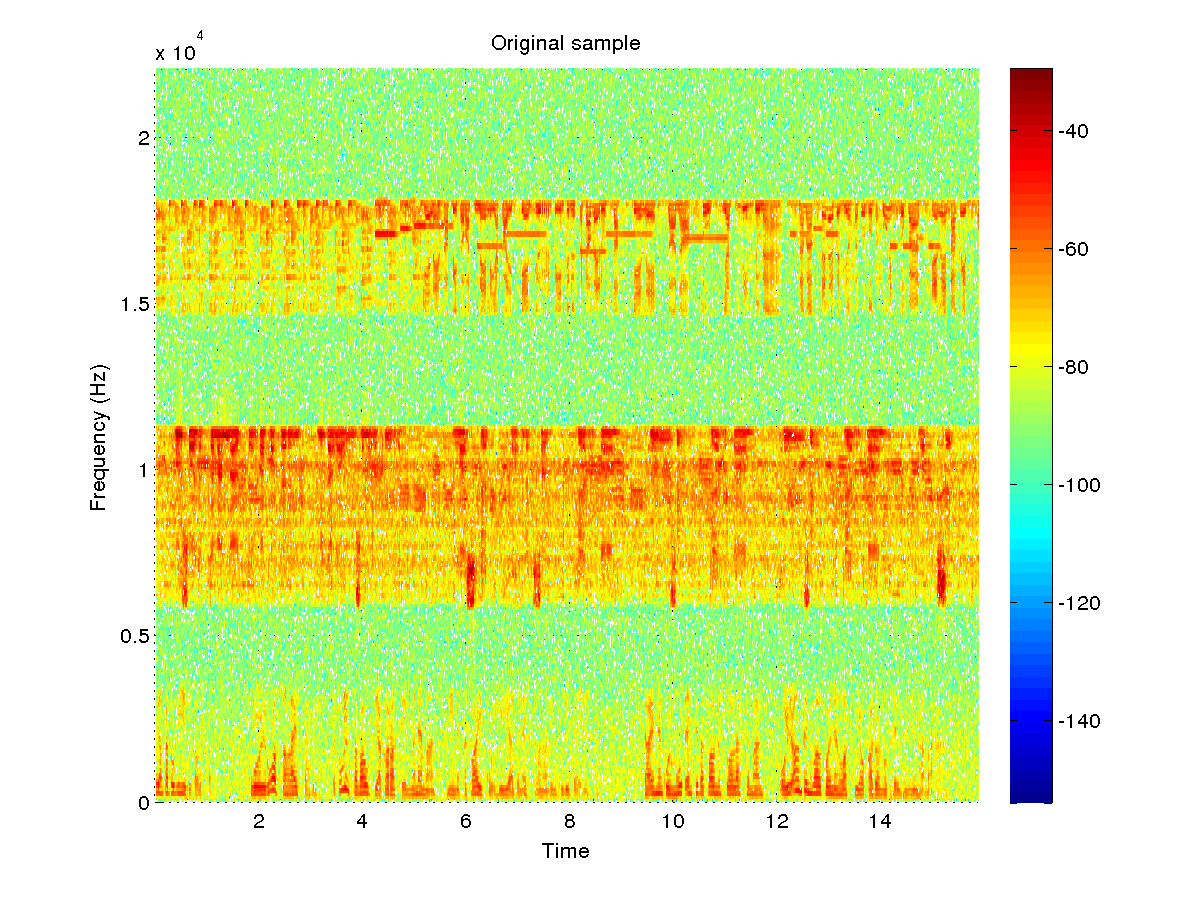
\includegraphics[width=180mm]{q1_spectrogram}
    \caption{Spectrogram of the signal. \label{fig:q1_spectrogram}}
  \end{center}  
\end{figure}

Assignment instructed the use of an IIR-filter with 500Hz transition
bands and maximum of 2 dB passband ripple.  The filter specification was
drawn with {\tt speksitIIR}, obtained from the course page.  The filter
specification is depicted in figure \ref{fig:q1_filter_specification}.

As the IIR filter, we chose Chebyshev type II, because of its good
features for the task at hand, i.e., non-existent ripple in the
passband.

The filtered signal's spectrogram is shown in figure
\ref{fig:q1_filtered_spectrogram}.

\begin{figure}
  \begin{center}
    \hspace*{-1in}
    \includegraphics[width=180mm]{q1_filter_specification}
    \caption{IIR filter specification for the
      passband. \label{fig:q1_filter_specification}}
  \end{center}  
\end{figure}

\begin{figure}
  \begin{center}
    \hspace*{-1in}
    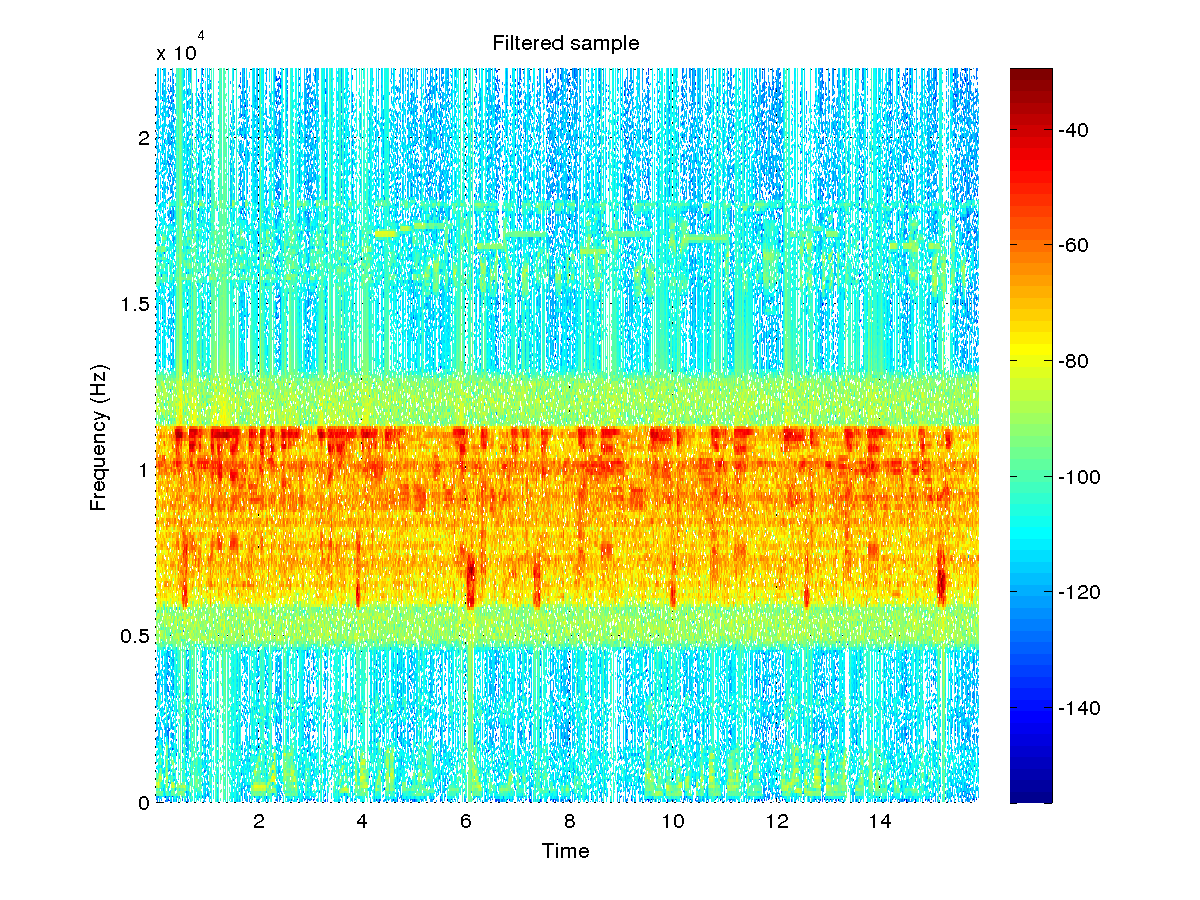
\includegraphics[width=180mm]{q1_filtered_spectrogram}
    \caption{Spectrogram of the filtered signal. 
      \label{fig:q1_filtered_spectrogram}}
  \end{center}  
\end{figure}

Demodulation was done as shown in Matlab round 5, with the following code
\begin{verbatim}
  x_demod = filtered .* cos(2*pi*fc/fT*[1:length(filtered)]');
\end{verbatim}

A nice frequency to perform the demodulation around, 11195 Hz, was found
after a few tries.  This gave a clear signal to listen to.

The sample contains two assignments: writing the song lyrics of the song
that can be heard when the sample is played backwards and the
calculation of ``8 * 6 * 6 * 2''.

The calculation produces the result 576.  The song lyrics can be heard
by using {\tt flipud}, and they are part of a song ``Tuntematon
potilas'' by Arttu Wiskari\cite{wiskari2010}.

\begin{quotation}
eikö aikani täynnä jo ois

olen jo nähnyt tämän elämän

kaiken sain ja vielä enemmän

kuule mun toive

mä haluan pois
\end{quotation}

Matlab code for the assignment is included in appendix \ref{sect:q1m}.


\section{Q2 DTMF}
DTMF is a signaling system that is used to
transmit numbers and characters. The original purpose of the system
was to transmit numbers entered by a caller.
The aim the exercise was to analyse a given DTMF signal by
creating a function which recognises the numbers in the signal
automatically.

The DTMF system works by sending signals at two different
frequencies. Each transmitted number corresponds to an unique
letter. For example the frequencies 770 Hz and 1336 Hz together
represent the number 5.

It was given in the exercise that each number is at least
70ms long and there is a pause of at least 40ms between each number. We
ended up using a 20ms sized window since this guarantees, that
there is at least one silent window between the numbers.
We differentiate the numbers using this silent window.

The flow of the program is as follows: for each window, the energy of the
window is calculated. If the energy exceeds a hard coded
threshold of 0.0001, we assume that the window constains an
actual signal. If the threshold is exceeded, we calculate
the amplitude response of the signal, an example of which is depicted in
figure \ref{fig:q2_amplitude_response}.


\begin{figure}[h!]
  \begin{center}
    \hspace*{-1in}
    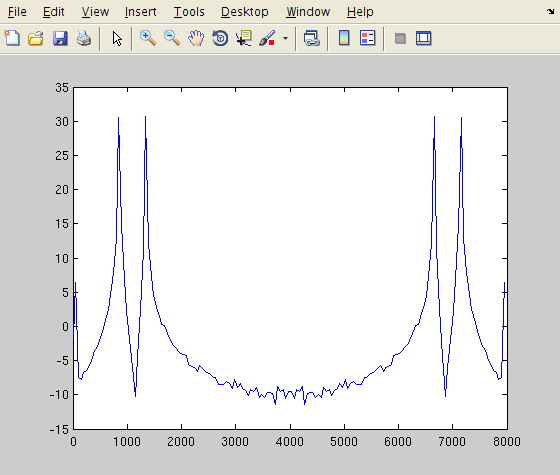
\includegraphics[width=100mm]{Q2/magnitude_vs_freq.png}
    \caption{The amplitude response of the signal. 
      \label{fig:q2_amplitude_response}}
  \end{center}  
\end{figure}


In the figure it is easy to see the two frequencies which
contain the information about the number being transmitted.
The program finds the two peaks scanning through the frequency spectrum
and taking the first value that exceeds the threshold, then scanning
ahead until the specturm goes under the threashold and then taking the
first value to exceed the threshold again. Then the program rounds
the two found frequencies to the nearest matching  DTMF frequency and
translates them into the corresponding number. Once the number has been
decoded, the program waits for the next silent window.

The program gave correct results for the given signal
\verb|dtmf_81231H-wav|,
but when it was tested with the 12 test signals,
it was only able to get 6 signals perfectly decoded.

It could be possible to improve the program by tuning the
hard coded thresholds better and using a more sophisticated
method for detecting the peaks. We could also
consider all 20ms windows
of the signal, not just the first one.



\clearpage

\addcontentsline{toc}{section}{\refname}  % article
\bibliographystyle{plain}
\bibliography{project_bibliography}

\end{document}
